\section[Ход работы]{ХОД РАБОТЫ}

\subsection{Описание предметной области}

В качестве предметной области данной расчетной работы были выбраны
описание и автоматизация учета данных бизнес-процессов спортивного магазина,
занимающегося реализацией экипировки для настольного тенниса.
Будем рассматривать следующие объекты предметной области:
\begin{itemize}
\item товар (ракетки, основания, накладки и шарики);
\item производители товара;
\item поставщики товара.
\end{itemize}

Определим следующие бизнес-процессы предметной области:
\begin{itemize}
\item поступление товара;
\item реализация товара.
\end{itemize}

Перечислим задачи, решаемые разрабатываемой системой:
\begin{itemize}
\item учет поступления и реализации товара;
\item предоставление информации на основе накопленных данных.
\end{itemize}

\subsection{Создание перечислений}

Создание перечислений производится с помощью раздела <<Перечисления>>
панели <<Конфигурация>> режима <<Конфигуратор>>.
Для создания перечисления необходимо, щелкнув правой кнопкой мыши по этому
разделу, выбрать пункт <<Добавить>>. Далее в появившемся окне
следует определить имя и синоним перечисления.
После этого в разделе <<Данные>> необходимо определить возможные значения
создаваемего перечисления.

В силу специфики предметной области удобно использовать следующие
перечисления для определения множества значений свойств товаров:
\begin{itemize}
\item <<КлассРакетки>> со значениями
  <<S1>> (синоним: <<*>>),
  <<S2>> (синоним: <<**>>),
  <<S3>> (синоним: <<***>>),
  <<S4>> (синоним: <<****>>),
  <<S5>> (синоним: <<*****>>);
\item <<КлассОснования>> со значениями
  <<OFFplus>> (синоним: <<OFF+>>),
  <<OFF>> (синоним: <<OFF>>),
  <<OFFminus>> (синоним: <<OFF->>),
  <<ALL>> (синоним: <<ALL>>),
  <<DEFplus>> (синоним: <<DEF+>>),
  <<DEF>> (синоним: <<DEF>>),
  <<DEFminus>> (синоним: <<DEF->>);
\item <<КлассШарика>> со значениями
  <<S1>> (синоним: <<*>>),
  <<S2>> (синоним: <<**>>),
  <<S3>> (синоним: <<***>>);
\item <<ЦветШарика>> со значениями
  <<Белый>> и
  <<Оранжевый>>.
\end{itemize}

На рисунке~\ref{fig:enum} в качестве примера приведены
значения перечисления <<КлассРакетки>> в интерфейсе конфигуратора
СКД 1C:Предприятие.

\begin{figure}[h!]
  \centering
  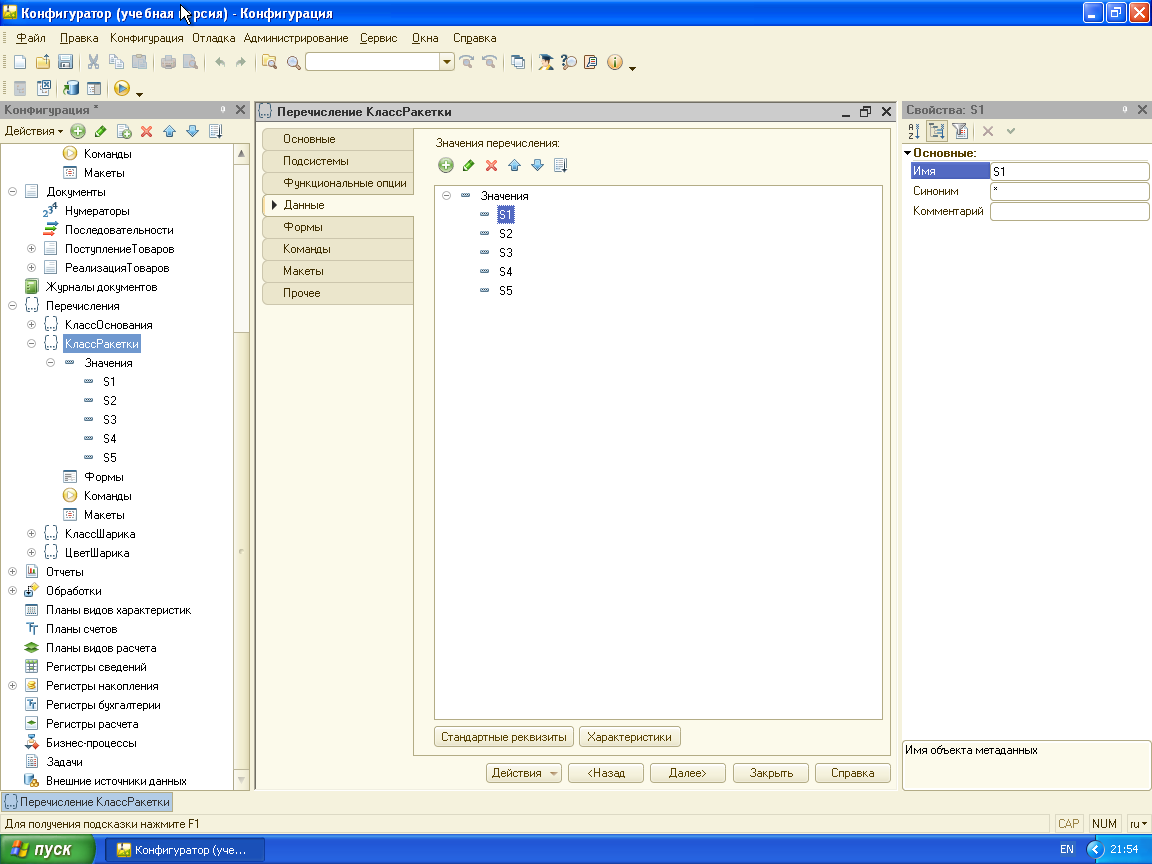
\includegraphics[width=130mm]{pic/enum}
  \caption{Значения перечисления <<КлассРакетки>>}
  \label{fig:enum}
\end{figure}

Созданные перечисления призваны сэкономить время и снизить количество
ошибок при заполнении справочников.

\subsection{Создание справочников}

Создание справочников производится с помощью раздела <<Справочники>>
панели <<Конфигурация>> режима <<Конфигуратор>>.
Для создания справочника необходимо, щелкнув правой кнопкой мыши по этому
разделу, выбрать пункт <<Добавить>>. Далее в появившемся окне
следует определить имя и синоним справочника.
После этого в разделе <<Данные>> необходимо определить структуру
хранимых данных путем добавления и указания свойств реквизитов
и табличных частей.

В разрабатываемой информационной системе справочники соответствуют
объектам предметной области: <<Производители>>, <<Поставщики>>,
<<Ракетки>>, <<Основания>>, <<Накладки>>, <<Шарики>>.

Структура справочника <<Производители>>:
\begin{itemize}
\item поле <<Наименование>>, вводимое вручную (длина: 25);
\item реквизит <<Страна>> (тип: строка, длина: 50);
\item реквизит <<Описание>> (тип: строка, длина: неограниченная).
\end{itemize}

Структура справочника <<Поставщики>>:
\begin{itemize}
\item поле <<Наименование>>, вводимое вручную (длина: 250);
\item реквизит <<ЮридическийАдрес>> (тип: строка, длина: 50);
\item табличная часть <<КонтактныеЛица>>, содержащая поля
  <<ФИО>> (тип: строка, длина: 50),
  <<Должность>> (тип: строка, длина: 50) и
  <<Номер телефона>> (тип: строка, длина: 20).
\end{itemize}

На рисунке~\ref{fig:sprav_postav} в качестве примера приведена
структура справочника <<Поставщики>> в интерфейсе конфигуратора
СКД 1C:Предприятие.

\begin{figure}[h!]
  \centering
  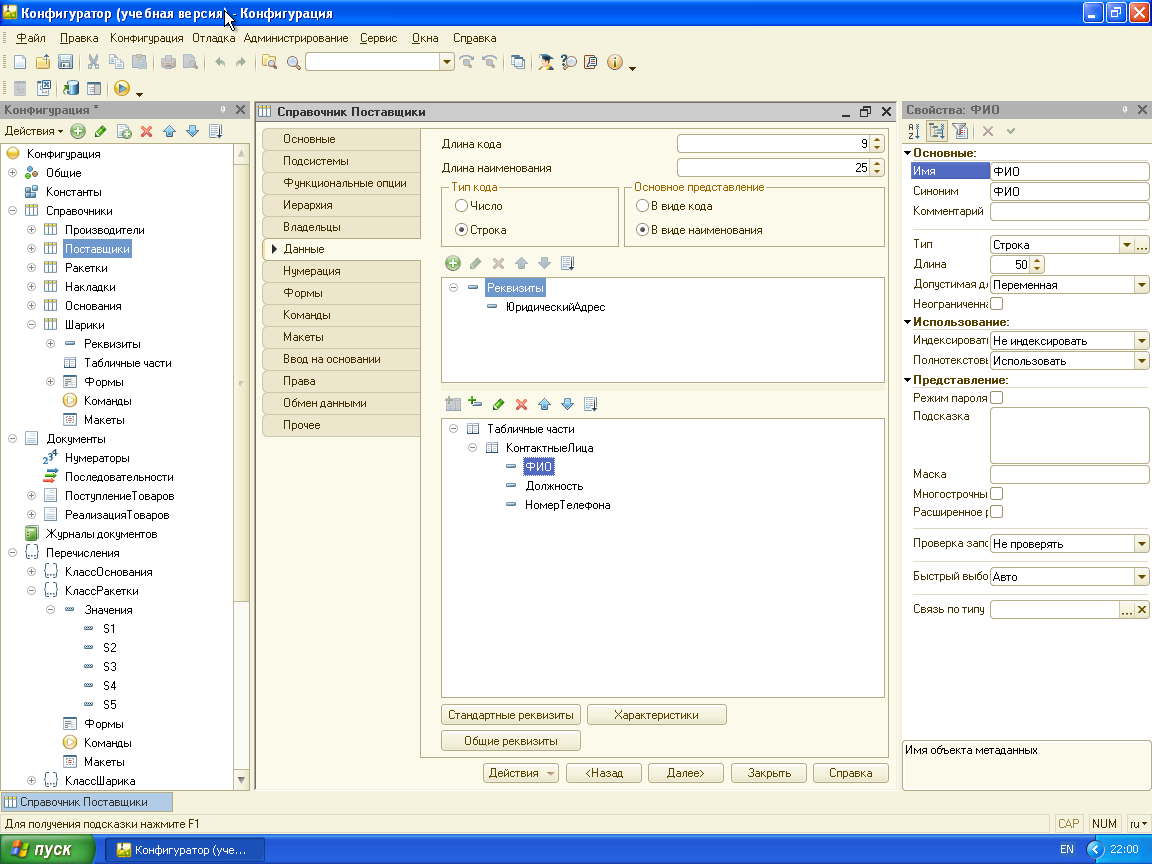
\includegraphics[width=130mm]{pic/sprav_postav}
  \caption{Структура справочника <<Поставщики>>}
  \label{fig:sprav_postav}
\end{figure}

\pagebreak

Структура справочника <<Ракетки>>:
\begin{itemize}
\item поле <<Наименование>>, формируемое автоматически (длина: 25);
\item реквизит <<Производитель>> (тип: <<СправочникСсылка.Производи-тели>>);
\item реквизит <<Модель>> (тип: строка, длина: 25);
\item реквизит <<Класс>> (тип: <<ПеречислениеСсылка.КлассРакетки>>);
\item реквизит <<Вес>> (тип: число).
\end{itemize}

Для того, чтобы значение поля <<Наименование>> справочника <<Ракетки>>
формировалось на основании значения реквизитов <<Производитель>> и <<Модель>>
автоматически, создадим форму ввода данных <<ВводДанных>>,
удалим с неё элемент ввода наименования, как показано на
рисунке~\ref{fig:sprav_auto_name} и назначим обработчики событий
<<ПроизводительПриИзменении>> и <<МодельПриИзменении>>,
как показано на рисунке~\ref{fig:sprav_auto_name_module}.

\begin{figure}[h!]
  \centering
  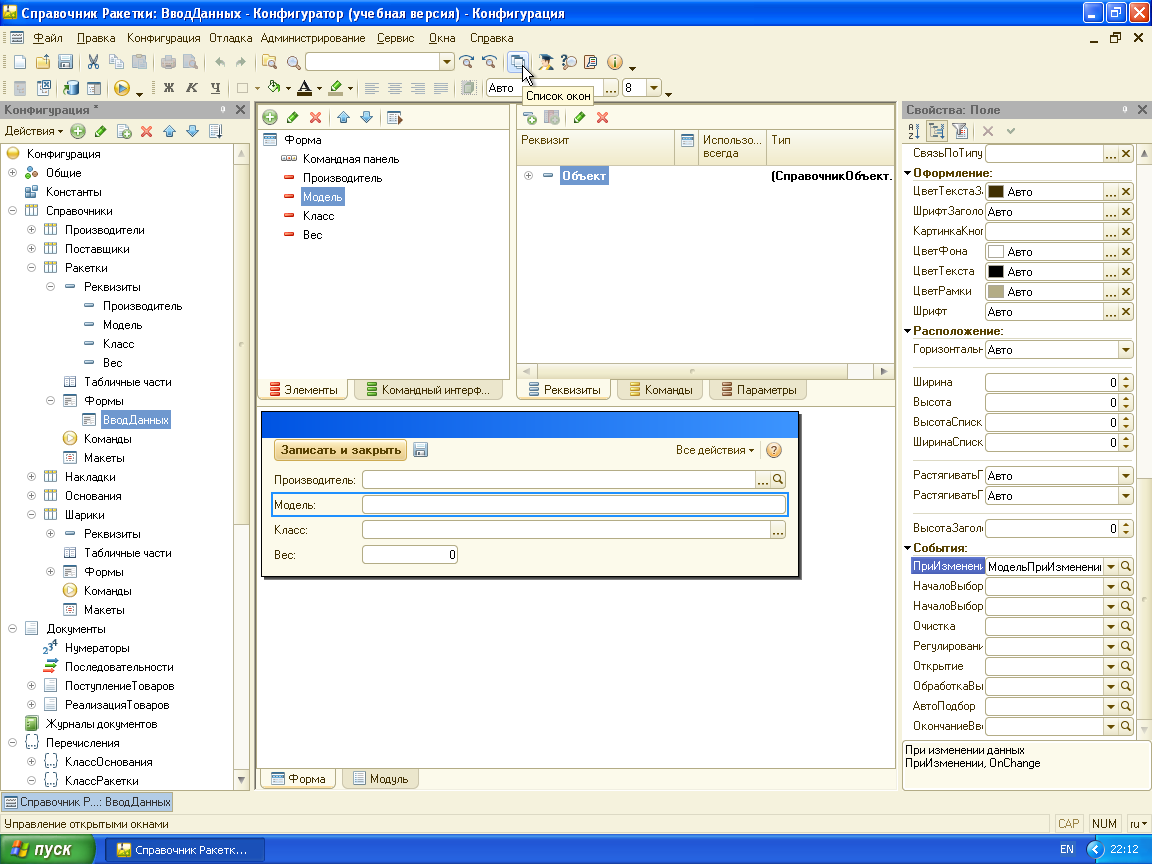
\includegraphics[width=130mm]{pic/sprav_auto_name}
  \caption{Модифицированная форма ввода данных \\ справочника <<Ракетки>>}
  \label{fig:sprav_auto_name}
\end{figure}

\begin{figure}[h!]
  \centering
  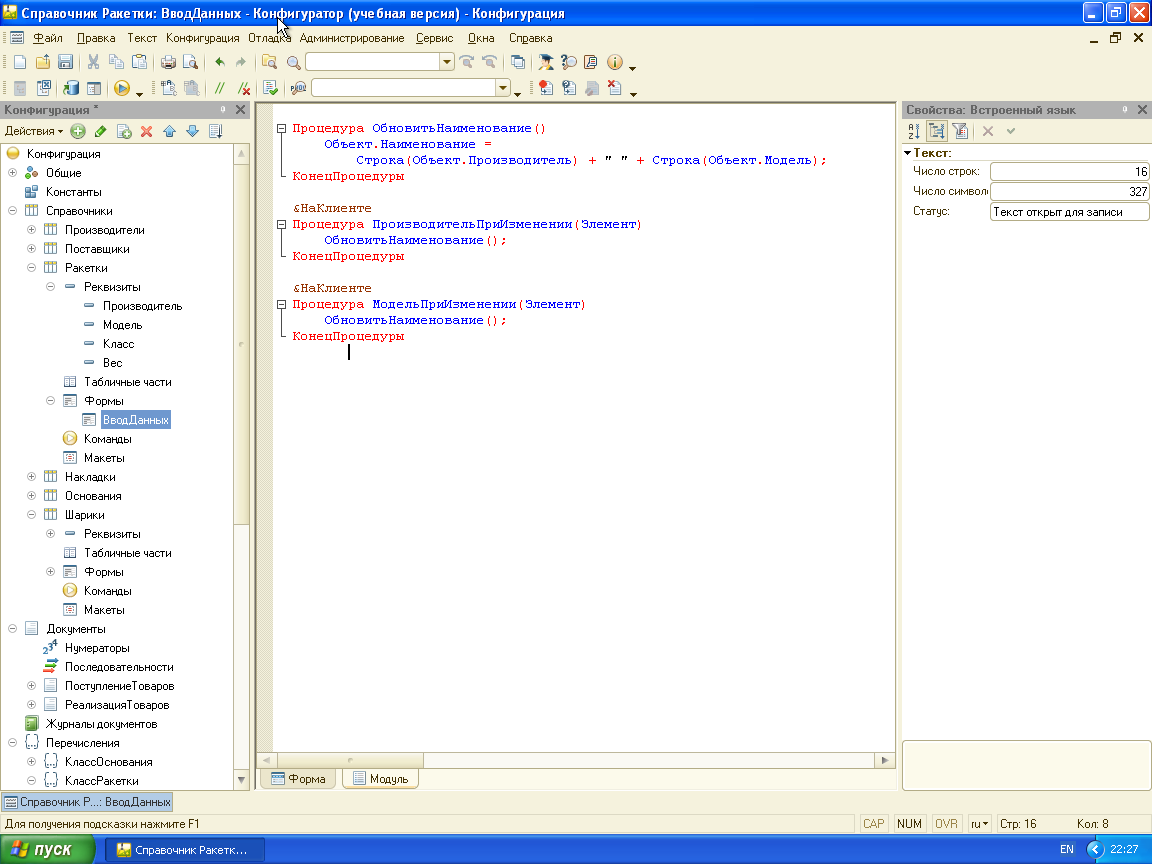
\includegraphics[width=130mm]{pic/sprav_auto_name_module}
  \caption{Обработчики событий формы ввода данных \\ справочника <<Ракетки>>}
  \label{fig:sprav_auto_name_module}
\end{figure}

Структура справочника <<Основания>>:
\begin{itemize}
\item поле <<Наименование>>, формируемое автоматически (длина: 25);
\item реквизит <<Производитель>> (тип: <<СправочникСсылка.Производи-тели>>);
\item реквизит <<Модель>> (тип: строка, длина: 50);
\item реквизит <<Класс>> (тип: <<ПеречислениеСсылка.КлассОснования>>);
\item реквизит <<Вес>> (тип: число).
\end{itemize}

Структура справочника <<Накладки>>:
\begin{itemize}
\item поле <<Наименование>>, формируемое автоматически (длина: 25);
\item реквизит <<Производитель>> (тип: <<СправочникСсылка.Производи-тели>>);
\item реквизит <<Модель>> (тип: строка, длина: 50);
\item реквизиты <<Скорость>>, <<Вращение>> и <<Контроль>>
  (тип: число, минимальное: 0, максимальное: 100).
\end{itemize}

Структура справочника <<Шарики>>:
\begin{itemize}
\item поле <<Наименование>>, формируемое автоматически (длина: 25);
\item реквизит <<Производитель>> (тип: <<СправочникСсылка.Производи-тели>>);
\item реквизит <<Класс>> (тип: <<ПеречислениеСсылка.КлассШарика>>);
\item реквизит <<Цвет>> (тип: <<ПеречислениеСсылка.Цвет>>).
\end{itemize}

Значение поля <<Наименование>> справочников <<Основания>>, <<Накладки>> и <<Шарики>>
формируется аналогично.

\subsection{Создание документов}

ПоступлениеТоваров

РеализацияТоваров

\subsection{Создание регистра накопления}

КоличествоТовара

\subsection{Создание отчетов}

Отчет по поступлению товаров

Отчет по реализации товаров

Статистика поступления товаров

\subsection{Создание запросов}

ДорогиеТоварыЗаанногоПоставщика

ДиректорыПоставщиков

РеализованныеТовары

ПоставкиТоваровИтоги

БалансПоставокИРеализацииТоваров

СтатистикаПоставок